% Created 2026-09-07 Mo 13:45
% Intended LaTeX compiler: pdflatex
\documentclass[presentation]{beamer}
\usepackage[utf8]{inputenc}
\usepackage[T1]{fontenc}
\usepackage{graphicx}
\usepackage{longtable}
\usepackage{wrapfig}
\usepackage{rotating}
\usepackage[normalem]{ulem}
\usepackage{amsmath}
\usepackage{amssymb}
\usepackage{capt-of}
\usepackage{hyperref}
\usepackage[style=authoryear,mincitenames=1,maxcitenames=2]{biblatex}
\usepackage[style=authoryear,mincitenames=1,maxcitenames=2]{biblatex}
\addbibresource{~/org/biblio/pop-gen.bib}
\setbeamerfont{caption}{size=\scriptsize}
\author[]{Philip Wolper \inst{1} \and Johannes Müller \inst{2} \and Aurélien Tellier \inst{1}}
\institute[]{\inst{1} Section of Population genetics, Technical University of Munich \and \inst{2} Department of Mathematics, Technical University of Munich}
\usetheme{Berlin}
\date{\today}
\title{Pathogen dynamics nested in a host Wright-Fisher model: towards joint host-pathogen genealogies}
\subtitle{CoNeMEsSA Seminar}
\hypersetup{
 pdfauthor={Philip Wolper},
 pdftitle={Pathogen dynamics nested in a host Wright-Fisher model: towards joint host-pathogen genealogies},
 pdfkeywords={},
 pdfsubject={},
 pdfcreator={Emacs 29.3 (Org mode 9.7.39)}, 
 pdflang={English}}
\begin{document}

\maketitle
\begin{frame}{Outline}
\tableofcontents
\end{frame}

\section{Phylodynamics}
\label{sec:org42ef6d1}
\begin{frame}[label={sec:org4da51e7}]{Phylodynamics: Inferring epidemiological parameters from pathogen genetic sequences.}
\begin{columns}
\begin{column}{0.5\columnwidth}
\begin{itemize}
\item Pathogens coalesce backwards in time with the transmission tree of infected individuals.
\item We can derive the coalescent rates from an epidemiological model (incidence and prevalence), and compare to observed pathogen sequence trees.
\end{itemize}
\end{column}
\begin{column}{0.5\columnwidth}
\begin{figure}[htbp]
\centering
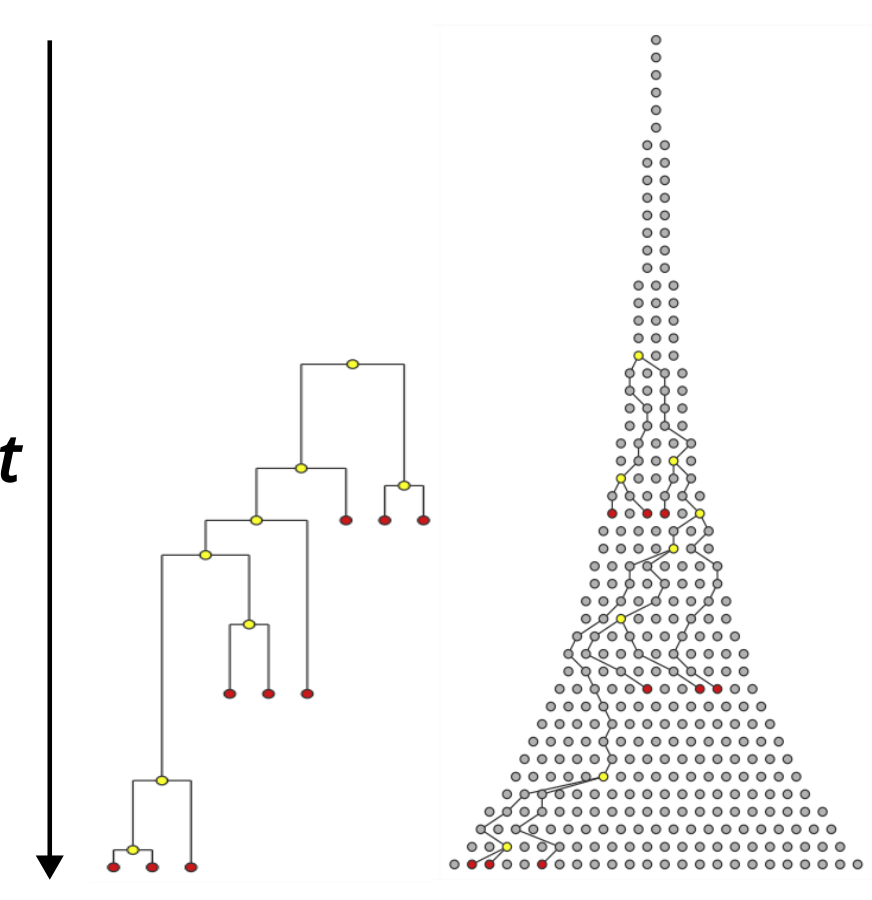
\includegraphics[width=0.8\textwidth]{./Kuehnert-infection_process.png}
\caption{Infectious branching process from \cite{kuehnert-2011-phylog-epidem}.}
\end{figure}
\end{column}
\end{columns}
\end{frame}
\begin{frame}[label={sec:orgaa00027}]{Phylodynamics: Basics of pathogen coalescence}
\begin{columns}
\begin{column}{0.45\columnwidth}
\begin{figure}[htbp]
\centering
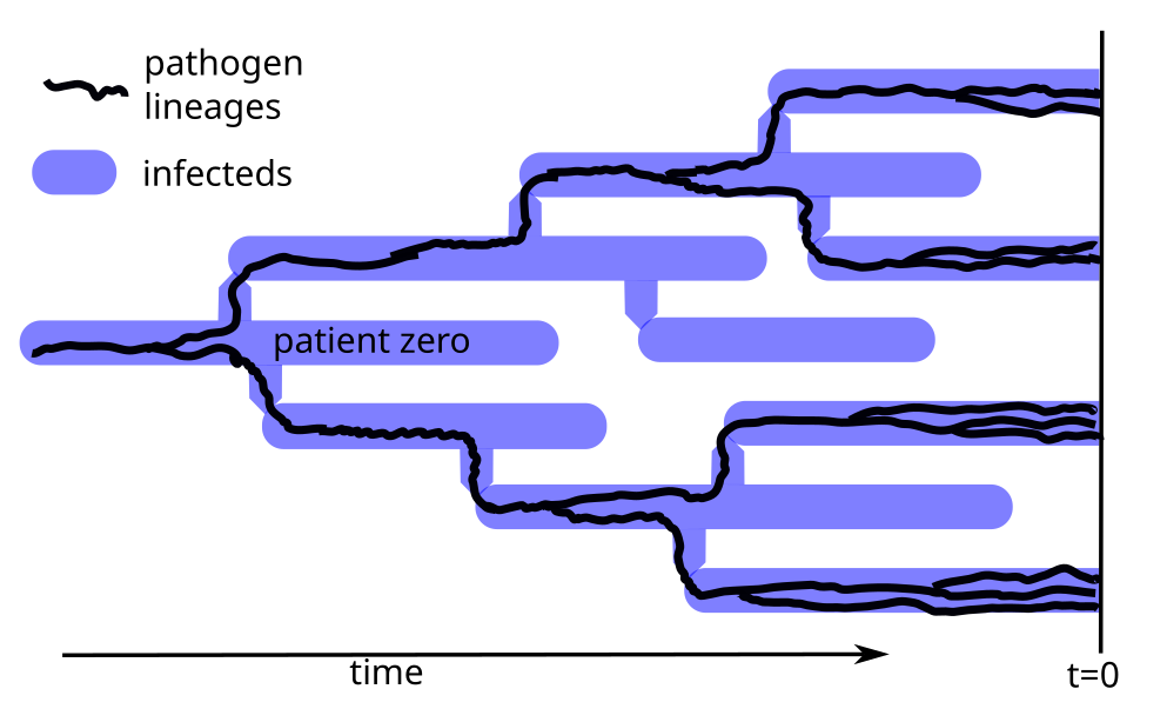
\includegraphics[width=\textwidth]{./Müller_EpiSkript_PhylodynamicsFig.png}
\caption{Pathogen coalescent within transmission tree (J. Müller, 2026)}
\end{figure}

\vspace{25pt}
\end{column}
\begin{column}{0.55\columnwidth}
\vspace{45pt}
\begin{figure}[htbp]
\centering
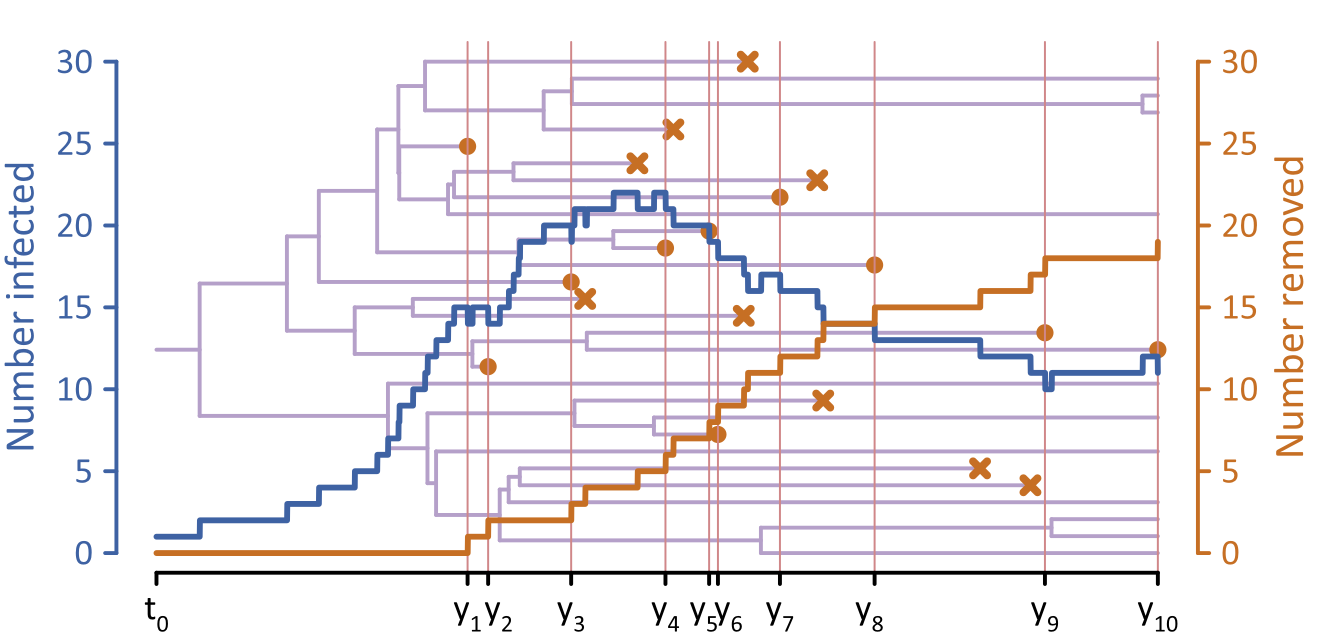
\includegraphics[width=\textwidth]{./plessis_2015_Fig1D.png}
\caption{Coalescent process within the epidemiological dynamics of \(I\) (Fig. 1D, \cite{plessis-2015-gettin-to})}
\end{figure}
\end{column}
\end{columns}
\end{frame}
\begin{frame}[label={sec:org3ff913e}]{Phylodynamics: Assumptions}
\begin{block}{Assumptions}
\begin{enumerate}
\item Host coalescence is neglegible compared to pathogen coalescent times.
\item Pathogen coalescent tree reflects the transmission tree.
\item Each host is infected by a single pathogen, so \(I \sim N_{\text{Pathogen}}\)
\item Evolution is measurable, i.e mutations occur on the timescale of transmission.
\end{enumerate}
\end{block}
\vspace{5pt}
\textbf{Real-world host-pathogen systems:}\\
\begin{itemize}
\item complex disease life-cycles including \emph{varying transmission modes}, vectors and environmental factors
\item reciprocal host-pathogen interactions (\emph{coevolution})
\end{itemize}
\end{frame}
\section{Joint Host-Pathogen Genealogies}
\label{sec:org068a886}
\begin{frame}[label={sec:org6499fb5}]{Joint Host and Pathogen Genealogies}
\begin{columns}
\begin{column}{0.6\columnwidth}
Applying phylodynamics to diseases beyond epidemic growth, requires consideration of host coalescence, i.e. \textbf{no} time scale separation of host and pathogen coalescence:\\

\vspace{30pt}

\textbf{The pathogen genealogical process is embedded within the host genealogy, mediated by horizontal and vertical transmission}\\
\end{column}
\begin{column}{0.45\columnwidth}
\begin{center}
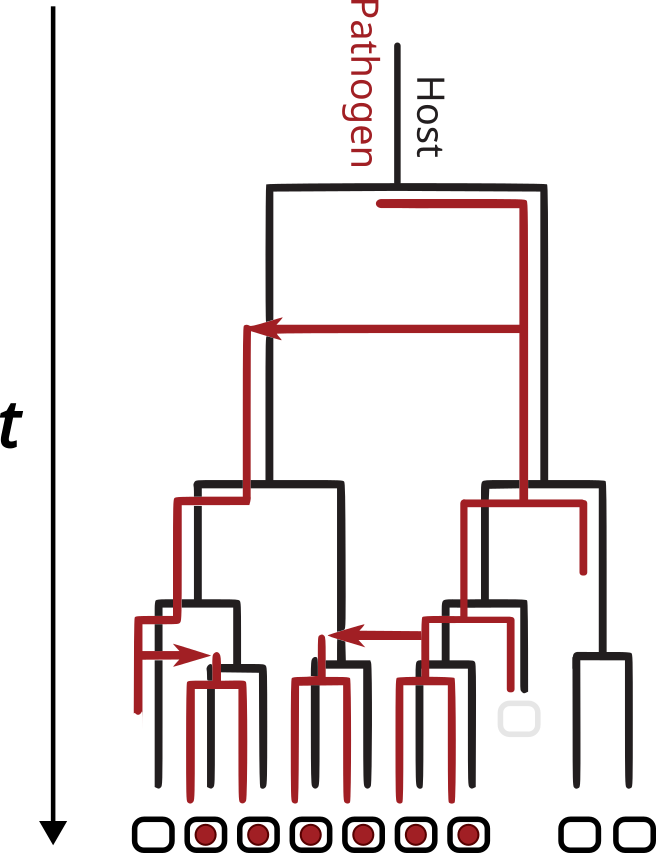
\includegraphics[width=.9\linewidth]{./nestedHostPathogenGenealogies.png}
\end{center}
\end{column}
\end{columns}
\end{frame}
\begin{frame}[label={sec:org0b715fb}]{Vertical and horizontal transmission}
\begin{columns}
\begin{column}{0.6\columnwidth}
\begin{exampleblock}{Transmission types}\label{sec:org80132ac}
\emph{\textbf{horizontal:}} \\
Infection dynamics driven by host-to-host transmission. eg. SI, epidemiological models.\\
\vspace{10pt}
\emph{\textbf{vertical:}} \\
Pathogen can be transmitted from infected hosts to their offspring \\
\vspace{5pt}
(eg. HIV, Hepatitis B/C, Zika, Toxoplasmosis, \ldots{})
\end{exampleblock}
\end{column}
\begin{column}{0.45\columnwidth}
\begin{center}
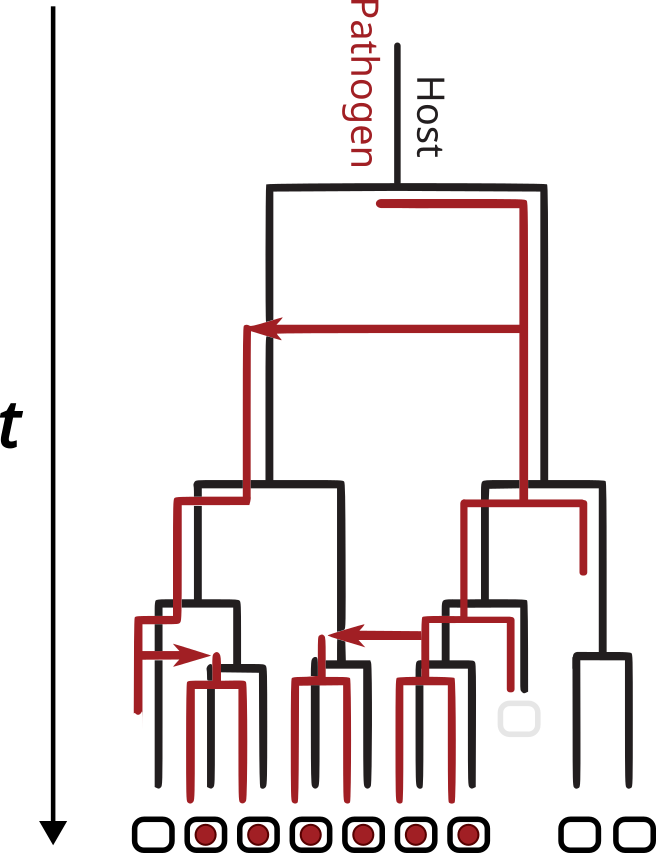
\includegraphics[width=.9\linewidth]{./nestedHostPathogenGenealogies.png}
\end{center}
\end{column}
\end{columns}
\end{frame}
\begin{frame}[label={sec:orgd0f1a7b}]{Existing work}
\begin{itemize}
\item \cite{lipsitch-1995-popul-dynam}: Epidemiological dynamics of vertical and horizontal transmission (but no coalescence\ldots{})
\end{itemize}

\vspace{10pt}

\begin{itemize}
\item \cite{welch-2005-integ-geneal-epidem}: Ancestral Infection and Selection Graph models joint host and pathogen genealogies within a Moran model framework.
\end{itemize}
\end{frame}
\begin{frame}[label={sec:org14b88f3}]{Our approach}
\begin{itemize}
\item Joint host and pathogen model with intertwined host and pathogen coalescence
\item Non-overlapping host generations (Wright-Fisher model)
\item Vertical pathogen transmission from one generation to the next
\item Epidemiological dynamics (SI model) within one host generation
\end{itemize}
\end{frame}
\section{Nested Host and Pathogen model}
\label{sec:org0160754}
\begin{frame}[label={sec:orgf71d89b}]{Semi-discrete nested Host-Pathogen model}
\begin{center}
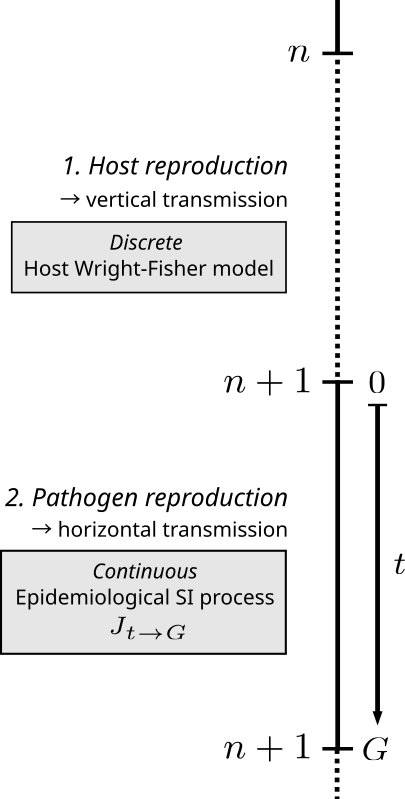
\includegraphics[width=0.3\textwidth]{./nestedHostPathogen_TimeScale.png}
\end{center}
\end{frame}
\begin{frame}[label={sec:org8b96ed3}]{Semi-discrete nested Host-Pathogen model}
\begin{center}
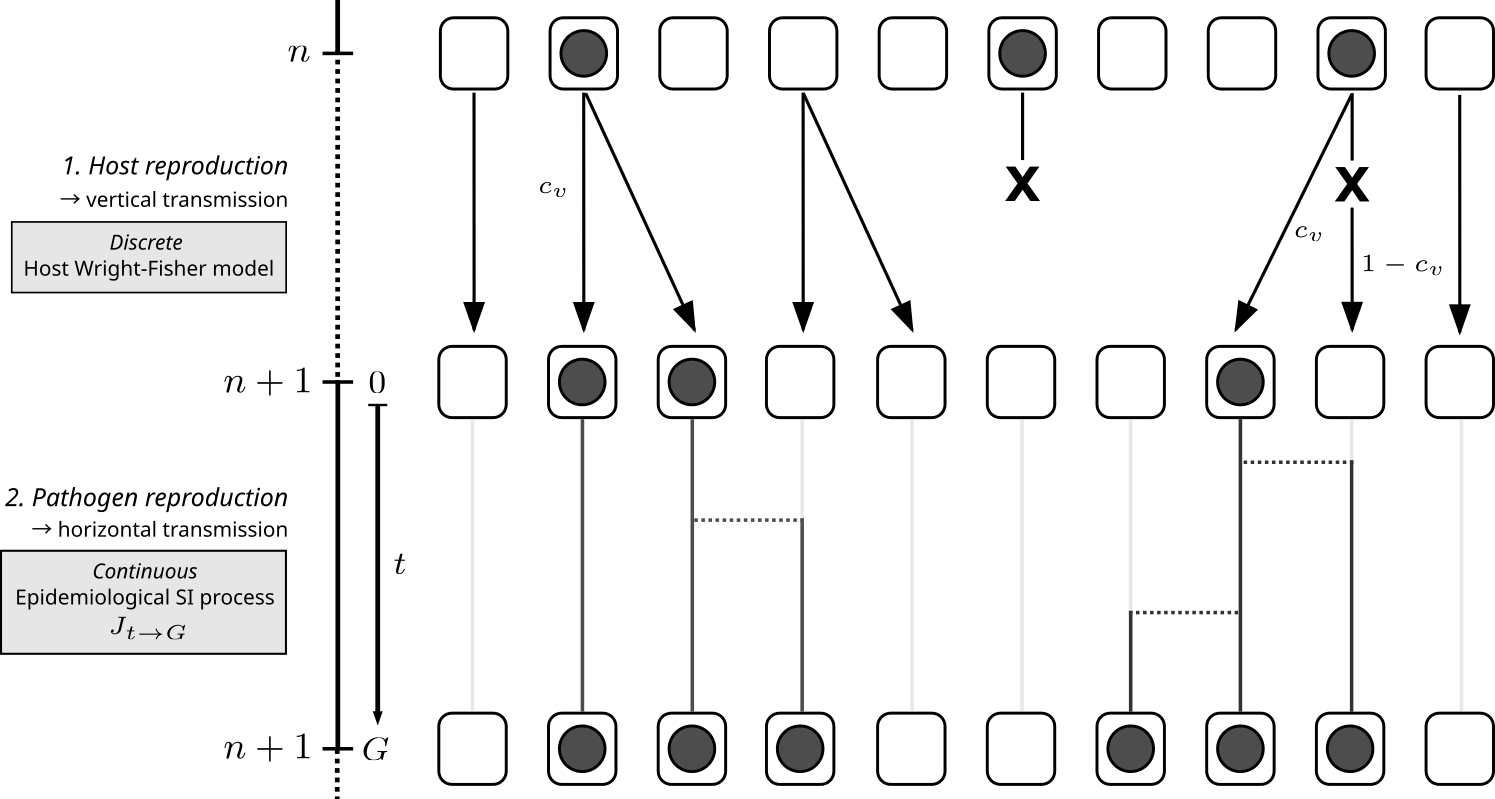
\includegraphics[width=.9\linewidth]{./nestedHostPathogen_WF_SI.png}
\end{center} 
\end{frame}
\begin{frame}[label={sec:orgbfa5b36}]{Bibliography}
\printbibliography
\end{frame}
\end{document}
